\section{Related Work}
\label{sec:related_work}

\paragraph{Automated Reasoning Dataset Construction.} 
Automated Dataset Construction (ADC) is essential for eliciting reasoning capabilities~\citep{liu2024automatic, wang2023data}. While most methods synthesize solvable puzzles~\citep{chen2025enigmata, NEURIPS2024_62ab1c2c} or verify rationale correctness~\citep{ling2023deductive, chen2025towards}, research into unsolvability remains limited. SQuAD 2.0~\citep{rajpurkar2018knowdontknowunanswerable} introduced unanswerable reading comprehension, while ReliableMath~\citep{xue2025reliablemathbenchmarkreliablemathematical} recently established unsolvable mathematics benchmarks and utilized SFT/DPO to enhance model performance in identifying flawed problems.

\begin{figure*}[t]
    \centering
    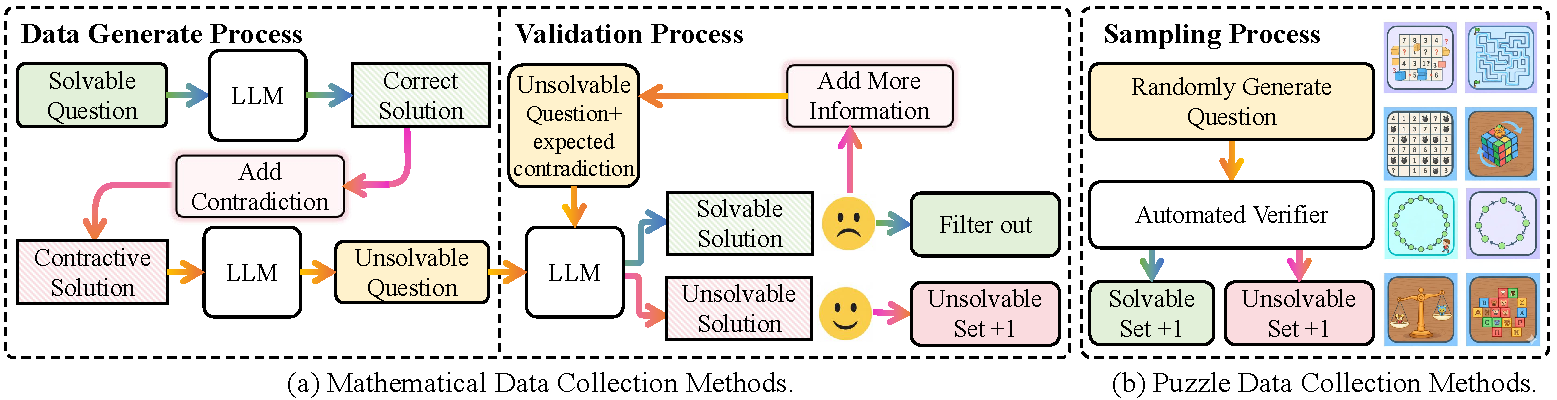
\includegraphics[width=\linewidth]{figures/data_con.pdf}
    \caption{The \textbf{UnsolvableQA} data collection pipeline. \textbf{(a) Mathematical Data:} We inject constraint conflicts into the solution paths of solvable problems via ``Reverse Construction,'' using LLM-based cross-verification and human auditing to validate the intended flaw. \textbf{(b) Puzzle Data:} Programmatic generators and deterministic verifiers (e.g., SAT solvers, DFS) rigorously classify generated instances into solvable and unsolvable sets.}
    \label{fig:pipeline}
\end{figure*}

\paragraph{Unanswerability Detection and Self-Awareness.} 
Recent interpretability research identifies that unanswerability is linearly encoded within an LLM's activation space, enabling binary detection via specific directions~\citep{lavi2025detecting}. Parallel studies on self-awareness and calibration~\citep{zhang2025self, mei2025reasoning, kalai2025languagemodelshallucinate, Steyvers2025} explore how models estimate subjective uncertainty and recognize knowledge boundaries to avoid hallucinations on difficult tasks.

\paragraph{Reinforcement Learning for Reasoning.} 
RL is central to aligning LLMs with complex reasoning~\citep{ouyang2022traininglanguagemodelsfollow, schulman2017proximalpolicyoptimizationalgorithms, rafailov2024directpreferenceoptimizationlanguage}. Algorithms like GRPO~\citep{shao2024deepseekmath} and DAPO~\citep{yu2025dapoopensourcellmreinforcement} significantly boost reasoning efficiency and capabilities~\citep{sheng2025hybridflow, tu2025learning, team2025kimi, guo2025deepseek, wang2025aspoasymmetricimportancesampling, chen2025aware}. To mitigate hallucinations, frameworks like TruthRL~\citep{wei2025truthrl} apply penalties to encourage models to refuse answering under uncertainty.

Despite these advancements, current paradigms exhibit three critical oversights. First, existing datasets primarily rely on shallow linguistic perturbations, lacking programmatically verifiable benchmarks with deep structural contradictions. Second, unsolvability detection remains a passive diagnostic tool for extractive tasks~\citep{lavi2025detecting}, lacking active alignment strategies to verbalize specific logical flaws. Finally, current RL frameworks conflate \textit{objective unsolvability} with \textit{subjective uncertainty}, which often triggers ``capability collapse'' through undifferentiated refusal. We bridge these gaps by systematically constructing inherently unsolvable data and establishing a robust three-way decision boundary: solving feasible tasks, explicitly detecting input-side answerability defects, and safely refusing queries beyond the model's capacity.